\documentclass[
%handout,notes=show
]{beamer}
%\usepackage{pgfpages}
%\setbeameroption{show notes on second screen}
%\setbeameroption{show only notes}
%\setbeameroption{show notes}

%\usepackage{pgfpages}
%\pgfpagesuselayout{4 on 1}[a4paper,border shrink=5mm]

%\mode<presentation>
\definecolor{pantone386c}{RGB}{98, 189, 25}
\setbeamercolor*{palette primary}{fg=white,bg=pantone386c}
\setbeamercolor*{palette secondary}{fg=white,bg=pantone386c}
\setbeamercolor*{palette tertiary}{fg=white,bg=pantone386c}
\setbeamercolor*{palette quaternary}{fg=white,bg=pantone386c}

\setbeamercolor*{titlelike}{fg=black}
%\setbeamercolor*{titlelike}{bg=pantone386c}
\setbeamercolor*{item}{fg=pantone386c}


% obs://home:lnussel/texlive-beamer-theme-Torino
%\usetheme{Torino}
%\usecolortheme{chameleon}
%\usetheme{Ilmenau}
%\usecolortheme[named=red]{structure}
\usefonttheme{structurebold}
%\useoutertheme{infolines}
%\useinnertheme{fancy}
%\setbeamertemplate{navigation symbols}{}
\beamertemplatenavigationsymbolsempty
%\usecolortheme{chameleon}

\usepackage{listings}
\usepackage{color}
%\usepackage[framemethod=tikz]{mdframed}

%\usepackage[firstpage]{draftwatermark}

\title{Overview of openQA}
\author[Ludwig Nussel]{Ludwig Nussel \texttt{<ludwig.nussel@suse.de>}}
\date{04.05.2015}
\institute[SUSE]{SUSE Linux GmbH}

\usepackage{listings}
\usepackage{pdfpages}

\lstdefinestyle{myperl}{
  language=Perl,
  showstringspaces=false,
  basicstyle=\footnotesize\ttfamily,
%  keywordstyle=\color{green}\ttfamily,
  stringstyle=\color{magenta}\ttfamily,
  commentstyle=\color{green}\ttfamily,
  morecomment=[l][\color{blue}]{\#}
}

\usebackgroundtemplate%
{%
  \vbox to \paperheight{\vfil 
\includegraphics[width=\paperwidth]{opensuse_waben_half}}%
}

\begin{document}

{
  \usebackgroundtemplate{}
  \setbeamercolor{background canvas}{bg=}
  \begin{frame}[plain]
    
\includepdf[pages=1]{template.pdf}
  \end{frame}
}

%\begin{frame}{Outline}
%  \tableofcontents
%%  % You might wish to add the option [pausesections]
%\end{frame}

\section{Intro}
\begin{frame}{Testing openSUSE releases ...}
  \begin{columns}[T]
    \column{.3\textwidth}
    \begin{itemize}
      \item NET images
      \item DVD images
      \item Live images
      \item Biarch DVD
      \item Rescue CD
    \end{itemize}
    \pause
    \column{.3\textwidth}
    \begin{itemize}
      \item USB
      \item DVD
      \item Desktop
      \item Laptop
      \item UEFI
      \item Legacy
    \end{itemize}
    \pause
    \column{.3\textwidth}
    \begin{itemize}
      \item GNOME
      \item KDE
      \item textmode
      \item RAID
      \item LVM
      \item ext4
      \item btrfs
      \item LUKS
      \item ...
    \end{itemize}
  \end{columns}
  \pause
  \textbf{... needs automation!}
\end{frame}

%\begin{frame}{Challenge}
%  \begin{itemize}
%    \item Packagers test their package but not the integration
%    \item Factory huge cauldron where one ingredient can spoil the soup
%      \note[item] { tw: 8000 packages, minimalx: 1000 packages }
%    \item too many install options to test manually
%      \note[item]{
%	DVD, NET, Live
%	64bit, 32bit
%	USB/DVD,btrfs/ext4
%      lvm/raid/encrypted,KDE/GNOME,dualboot,upgrade}
%    \item OBS builds ISOs at high rate
%  \end{itemize}
%\end{frame}

\section{openQA}

\begin{frame}{Basic Ideas}
  \begin{itemize}
    \item test full stack: bootloader, installer, desktop, apps
    \item use image recognition to "see like a human"
    \item act (keyboard, mouse) on the image seen
    \item use virtualization
    \item parallelize
    \item report!
  \end{itemize}
\end{frame}


\begin{frame}{Architecture}
  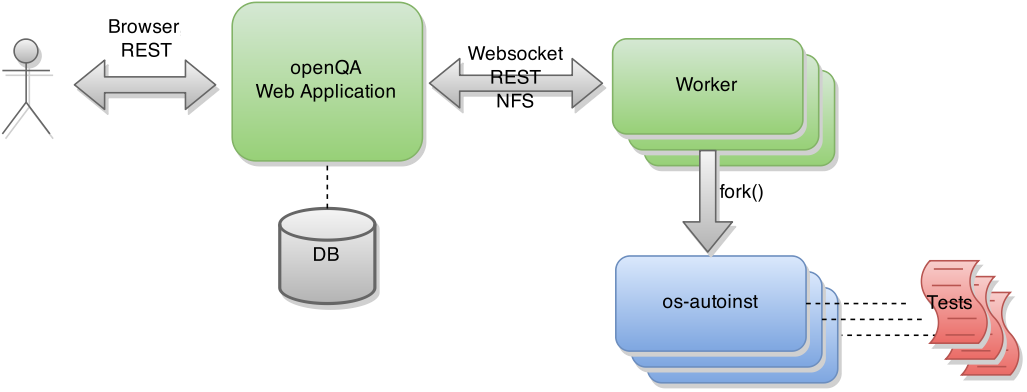
\includegraphics[width=.8\paperwidth]{openqa_architecture}
\end{frame}

\begin{frame}{openQA in openSUSE}
  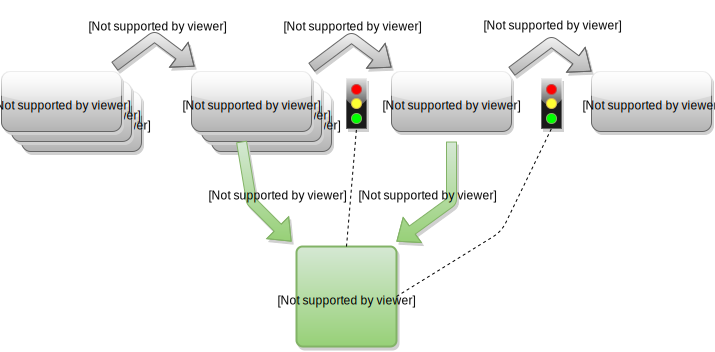
\includegraphics[width=.8\paperwidth]{openqa_in_devel_workflow}
\end{frame}

%\begin{frame}{Use Cases}
%  \begin{itemize}
%    \item OS installation
%    \item OS upgrade
%    \item regression testing
%    \item application testing
%    \item marketing, documentation
%  \end{itemize}
%\end{frame}

\begin{frame}{A Job in openQA}
  A job ...
  \begin{itemize}
    \item is a set of tests to run
    \item has a state (running, scheduled, cancelled, ...)
    \item has a result (passed, failed)
    \item has settings
    \begin{itemize}
      \item machine settings (disk size, CPU, ...)
      \item media/product settings (ISO name, repo to use, ...)
      \item test suite settings (Desktop, partitioning, ...)
    \end{itemize}
  \end{itemize}
\end{frame}

\begin{frame}{openQA welcome screen}
  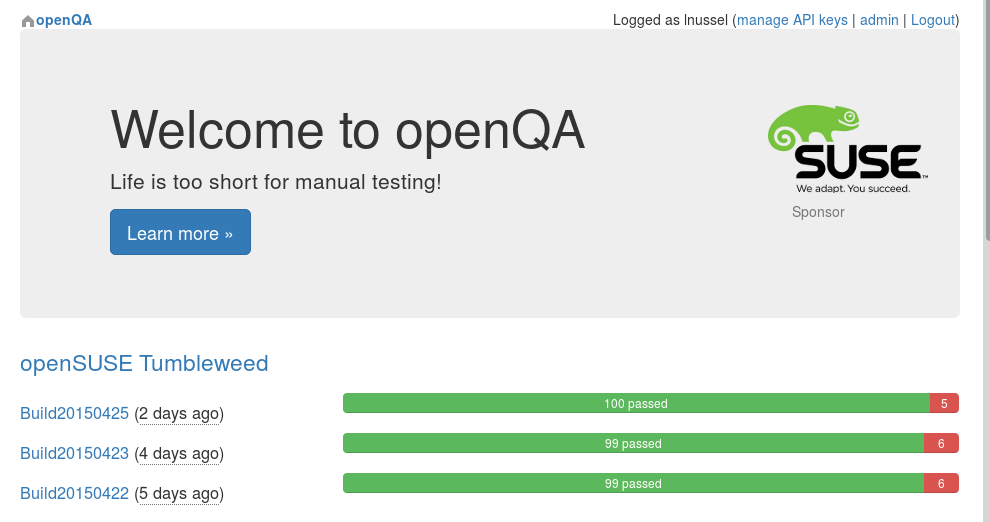
\includegraphics[width=.8\paperwidth]{openqa.png}
\end{frame}

\begin{frame}{openQA build overview}
  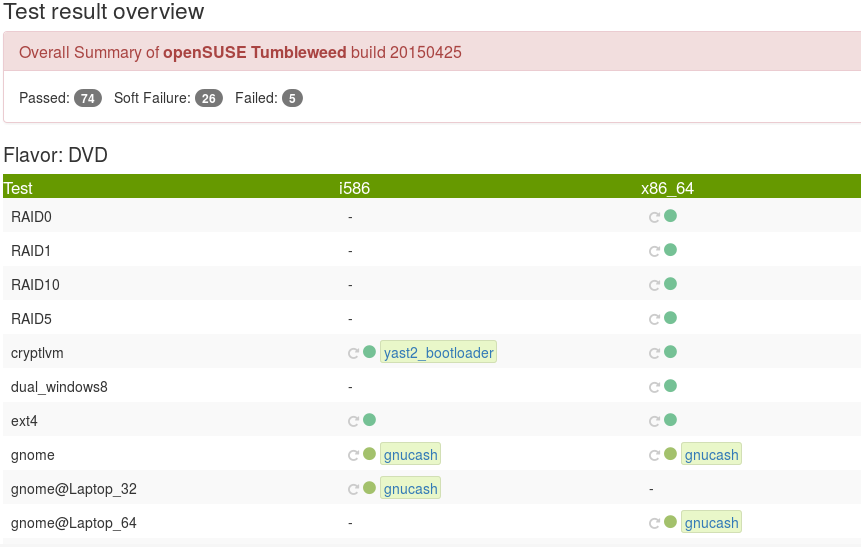
\includegraphics[width=.8\paperwidth]{openqa-buildoverview.png}
\end{frame}

\begin{frame}{openQA test results}
  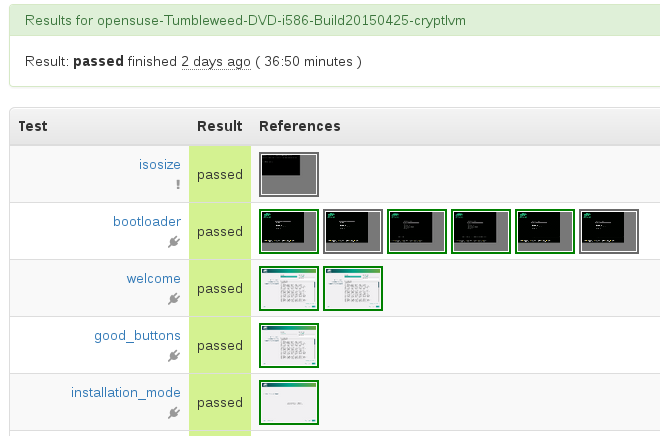
\includegraphics[width=.8\paperwidth]{openqa-testresults.png}
\end{frame}

\begin{frame}{openQA test result details }
  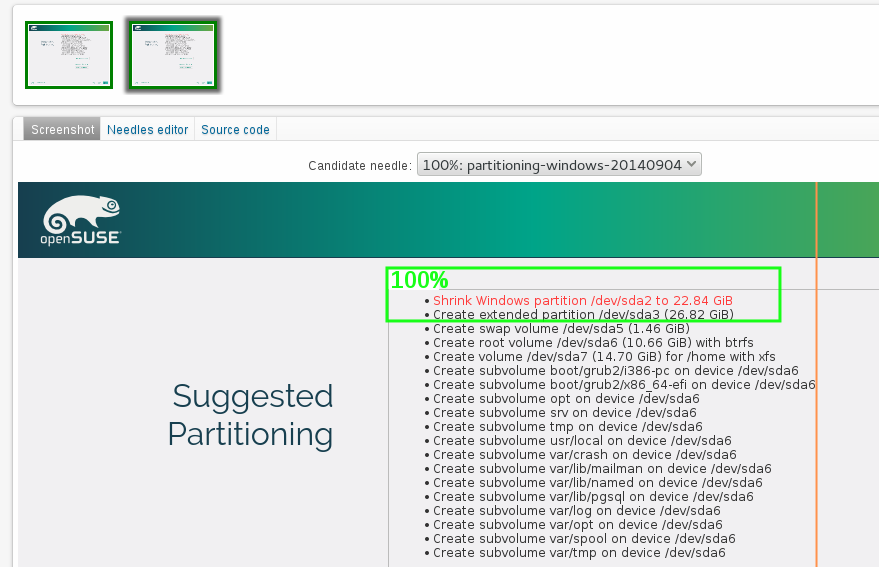
\includegraphics[width=.8\paperwidth]{openqa-match.png}
\end{frame}

%\begin{frame}{Needle matching}
%  \begin{itemize}
%    \item rectangular area in a screenshot
%    \item an area can be 'match' or 'exclude'
%      \note[item] {exclude area is useful for example to not try to match the clock which changes all the time obviously}
%    \item list of tags
%      \note[item] { needles are looked up by tags and tags are also used to filter out unwanted needles, e.g. gnome ones when testing KDE
%      }
%  \end{itemize}
%\end{frame}

\begin{frame}{Needle Editor}
  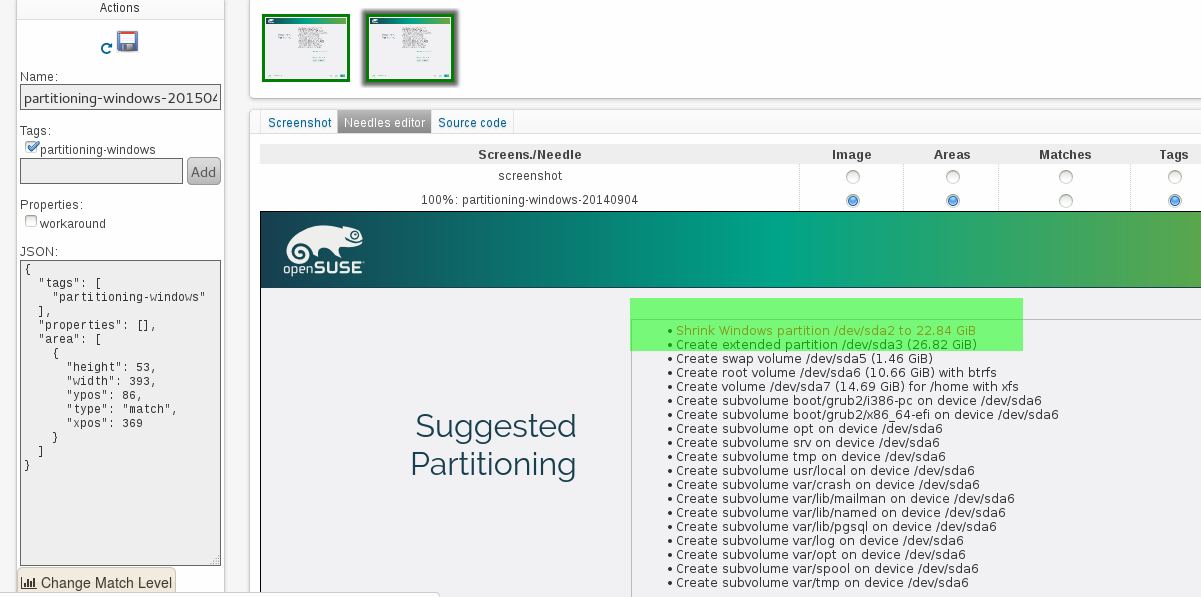
\includegraphics[width=.8\paperwidth]{openqa-needle-editor.png}
\end{frame}


%\begin{frame}{Templates}
%  describe products/jobs/machines job groups
%\end{frame}

\begin{frame}[fragile]{Test API}
  \lstset{style=myperl}
  \begin{lstlisting}
use base "basetest";
use strict;
use testapi;

sub run {
    # wait for bootloader to appear
    assert_screen "bootloader", 30;

    # "Install" is second option
    if (!get_var('LIVETEST')) {
      send_key "down";
    }

    # press enter to boot current entry
    send_key "ret";

    # wait for the desktop to appear
    assert_screen "desktop", 300;
}
  \end{lstlisting}
  % show get_var
  \note{As everything in openQA, tests are written in perl. No in depth
  knowledge of perl is requried though. The testapi module provides a simple
  and straight forward API for test developers.}
\end{frame}

\begin{frame}{Advanced Features}
  \begin{itemize}
    \item interactive needling mode
    \item real hardware testing
    \item multi machine support
  \end{itemize}
\end{frame}

\begin{frame}{Future Plans}
  \begin{itemize}
    \item disk images, autoyast profiles etc as result
    \item enhance multi machine networking
    \item even more support for hardware testing
    \item get rid of NFS
    \item more application testing
    \item do actual releases
  \end{itemize}
\end{frame}

\begin{frame}{Summary}
  \begin{itemize}
    \item state of the art web app
    \item test framework for fully automated OS and application testing
    \item visual documentation of test result, including video
       \note[item]{openQA saves the screenshots and records which image
       matched. So it's easy to see where and why a test failed}
    \item log files for failures
    \item simple API for tests
    \item remote controllable via REST API
  \end{itemize}
\end{frame}

\begin{frame}{Get it}
  \begin{description}
    \item[Web site] \url{http://os-autoinst.github.io/openQA/}
    \item[Code] \url{https://github.com/os-autoinst}
      \begin{description}
	\item[openQA] documentation, server, worker
	\item[os-autoinst] isotovideo tool and the API for tests.
	\item[os-autoinst-distri-opensuse] openSUSE tests
	\item[os-autoinst-needles-opensuse] openSUSE needles
      \end{description}
    \item[RPMs] \scriptsize{\url{https://build.opensuse.org/project/show/devel:openQA}}
  \end{description}
\end{frame}

\begin{frame}{Contact}
  \begin{itemize}
    \item openSUSE project management tool \url{https://progress.opensuse.org/projects/openqav3}
    \item \texttt{\#openSUSE-factory} IRC channel at Freenode
    \item \texttt{opensuse-factory@opensuse.org}
  \end{itemize}
\end{frame}

{
  \usebackgroundtemplate{}
  \setbeamercolor{background canvas}{bg=}
  
\includepdf[pages=2]{template.pdf}
  
\includepdf[pages=3]{template.pdf}
  
\includepdf[pages=4]{template.pdf}
}


% TODO: collect numbers, how many tests, duration etc.

\end{document}

%% vim: sw=2
